 %%%  Ukázkový text a dokumentace stylu pro text závěrečné (bakalářské a
%%%  diplomové) práce na KI PřF UP v Olomouci
%%%  Copyright (C) 2012 Martin Rotter, <rotter.martinos@gmail.com>
%%%  Copyright (C) 2014 Jan Outrata, <jan.outrata@upol.cz>


%%  Pro získání PDF souboru dokumentu je třeba tento zdrojový text v
%%  LaTeXu přeložit (dvakrát) programem pdfLaTeX.

%%  V případě použití programu BibLaTeX pro tvorbu seznamu literatury
%%  je poté ještě třeba spustit program Biber s parametrem jméno
%%  souboru zdrojového textu bez přípony a následně opět (dvakrát)
%%  přeložit zdrojový text programem pdfLaTeX.

%%  Postup získání Postscriptového souboru je popsán v dokumentaci.


%%  Třída dokumentu implementující styl pro závěrečnou práci. Vybrané
%%  nepovinné parametry (ostatní v dokumentaci):

%%  'master' pro sazbu diplomové práce, jinak se sází bakalářská práce

%%  'field=kód' pro Váš studijní obor, kódy pro diplomovou práci 'uvt'
%%  pro Učitelství výpočetní techniky pro střední školy a 'binf' pro
%%  Bioinformatiku, jinak je výchozí Informatika, a pro bakalářskou
%%  práci 'ainfk' pro Aplikovanou informatiku v kombinované formě,
%%  'inf' pro Informatiku, 'infv' pro Informatiku pro vzdělávání a
%%  'binf' pro Bioinfomatiku, jinak je výchozí Aplikovaná informatika
%%  v prezenční formě

%%  'printversion' pro sazbu verze pro tisk (nebarevné logo a odkazy,
%%  odkazy s uvedením adresy za odkazem, ne odkazy do rejstříku),
%%  jinak verze pro prohlížeč

%%  'biblatex' pro zapnutí podpory pro sazbu bibliografie pomocí
%%  BibLaTeXu, jinak je výchozí sazba v prostředí thebibliography

%%  'language=jazyk' pro jazyk práce, jazyky english pro anglický,
%%  slovak pro slovenský, jinak je výchozí czech pro český

%%  'font=sans' pro bezpatkový font (Iwona Light), jinak výchozí
%%  patkový (Latin Modern)

\documentclass[
%  master,
  field=ainfp,
%  printversion,
  master=true,
  biblatex,
  sourcecodes=false,
  theorems=false,
%  language=english,
%  font=sans,
  glossaries,
  index
]{kidiplom}

%% Informace pro úvodní strany. V jazyku práce (pokud není v komentáři
%% uvedeno česky) a anglicky. Uveďte všechny, u kterých není v
%% komentáři uvedeno, že jsou volitelné. Při neuvedení se použijí
%% výchozí texty. Text pro jiný než nastavený jazyk práce (nepovinným
%% parametrem language makra \documentclass, výchozí český) se zadává
%% použitím makra s uvedením jazyka jako nepovinného parametru.

%% Název práce, česky a anglicky. Měl by se vysázet na jeden řádek.
\title{Prolamování CAPTCHA zabezpečení}
\title[english]{Breaking the CAPTCHA}

%% Volitelný podnázev práce, česky a anglicky. Měl by se vysázet na
%% jeden řádek. Výchozí je prázdný.
% \subtitle{Ukázkový text a dokumentace stylu v \LaTeX{}u}
% \subtitle[english]{Sample text and documentation of the \LaTeX{} style}

%% Jméno autora práce. Makro nemá nepovinný parametr pro uvedení
%% jazyka.
\author{Bc. Kamil Hanus}

%% Jméno vedoucího práce (včetně titulů). Makro nemá nepovinný
%% parametr pro uvedení jazyka.
\supervisor{\\Mgr. Martin Trnečka, Ph.D.}

%% Volitelný rok odevzdání práce. Výchozí je aktuální (kalendářní)
%% rok. Makro nemá nepovinný parametr pro uvedení jazyka.
%\yearofsubmit{\the\year}

%% Anotace práce, včetně anglické (obvykle překlad z jazyka
%% práce). Jeden odstavec!
\annotation{Výsledkem práce je webová aplikace demonstrující vliv různých grafických operací na segmentaci symbolů z obrazu. Zároveň prolamuje známé druhy CAPTCHA kódů.}

\annotation[english]{Result of this thesis is web application presenting influence of different graphical operations to character segmentation from image. Application also breaks known types of CAPTCHA codes.}

%% Klíčová slova práce, včetně anglických. Oddělená (obvykle) středníkem.
\keywords{strojové učení; prolamování CAPTCHA}
\keywords[english]{machine learning; breaking CAPTCHA}

%% Volitelná specifikace příloh textu práce, i anglicky. Výchozí je '1
%% CD/DVD'.
%\supplements{jedno kulaté placaté CD/DVD s malou kulatou dírou uprostřed}
%\supplements[english]{one round flat CD/DVD with a small round hole in the middle}

%% Volitelné poděkování. Stručné! Výchozí je prázdné. Makro nemá
%% nepovinný parametr pro uvedení jazyka.
\thanks{Děkuji trpělivým.}

%% Cesta k souboru s bibliografií pro její sazbu pomocí BibLaTeXu
%% (zvolenou nepovinným parametrem biblatex makra
%% \documentclass). Použijte pouze při této sazbě, ne při (výchozí)
%% sazbě v prostředí thebibliography.
\bibliography{bibliografie.bib}

%% Další dodatečné styly (balíky) potřebné pro sazbu vlastního textu
%% práce.
\usepackage{lipsum}
\usepackage{verbatimbox}
\usepackage{subcaption} 
\usepackage{float}
\usepackage[inline]{enumitem}
\usepackage[]{algorithm2e}

\begin{document}
%% Sazba úvodních stran -- titulní, s bibliografickými údaji, s
%% anotací a klíčovými slovy, s poděkováním a prohlášením, s obsahem a
%% se seznamy obrázků, tabulek, vět a zdrojových kódů (pokud jejich
%% sazba není vypnutá).
\maketitle

%% Vlastní text závěrečné práce. Pro povinné závěry, před přílohami,
%% použijte prostředí kiconclusions. Povinná je i příloha s obsahem
%% přiloženého CD/DVD.

%% -------------------------------------------------------------------

\newcommand{\BibLaTeX}{\textsc{Bib}\LaTeX}
\renewcommand\UrlFont{}



\section{Úvod}
V posledních letech urazila technologie strojového učení a umělé inteligence velký posun vpřed. Ačkoliv historie vzniku termínu strojové učení sahá do  60. let 20. století, masová adaptace nastává až v posledních několika letech, kdy se lze s~pojmy umělá inteligence či AI (z anglického \textit{artificial intelligence})\footnote{\url{https://bit.ly/2KHOIiG}} setkávat stále častěji. Můžeme se domnívat, že jistou spojitost s nárůstem zájmu o strojové učení má i zpřístupnění open-source nástrojů, umožňujících snadnou aplikaci příslušných algoritmů, široké veřejnosti\footnote{\url{https://bit.ly/2z7TLCo}}.

Cílem této diplomové práce je vytvořit stručný přehled možností dnes hoj\-ně používaného CAPTCHA zabezpečení. Zároveň je k vybraným typům CAPTCHA zabezpečení navržena metoda umožňující jejich prolamování, jejíž úspěšnost je zároveň možné ověřit.  Aktuálně dostupné nástroje strojového učení poskytují elegantní způsob jak prolamovat klasické CAPTCHA zabezpečení. Zřejmě proto lze pozorovat vývoj nových typů CAPTCHA zabezpečení, které využívají ně\-kte\-ré prvky umělé inteligence. Diplomovou práci lze rozdělit do dvou částí. První se~zabývá samotným problémem CAPTCHA zabezpečení, jeho historií a možným prolamováním. Druhá popisuje aplikaci nazvanou CaptchaBreaker, vytvořenou v rámci této diplomové práce, která demonstruje možnost jak lze v rozumném čase řešit problém dekódování některých typů CAPTCHA kódů.
\newpage
\section{Captcha}
\subsection{Historie}
Za akronymem CAPTCHA je skryt anglický text \uv{\textbf{C}ompletely \textbf{A}utomated \textbf{P}ub\-lic \textbf{T}uring test to tell \textbf{C}omputers and \textbf{H}umans \textbf{A}part}. Obecně je principem testu vygenerování určitého typu dotazu a následné ověření odpovědi. Typicky se technologie využívá ve formulářích webových stránek. Na základě verifikace odpovědi je rozhodnuto, zda systém komunikuje s reálným uživatelem nebo robotem. Některé zdroje\footnote{\url{https://cs.wikipedia.org/wiki/CAPTCHA}} uvádějí pouze přepis textu z deformovaného obrazu do vstupního pole, což lze považovat za zavádějící, jelikož existuje několik dalších  variant. 

Důvod pro aplikaci takové ochrany je prostý. Pokud je umožněno na web zaslat libovolné požadavky bez omezení (například příspěvky do diskuzních fór, zakládání uživatelských účtů, pokusy o přihlášení, atd.), lze očekávat využití příležitosti útočníkem, který začne systém zahlcovat s úmyslem zamezit přístupnosti či šíření spamu. Ovšem je nutné mít na paměti, že nutnost prokazovat svou autentičnost je pro uživatele snížením komfortu. Proto se objevují technologie, které se snaží omezit interakci s uživatelem na minimum. 

Zajímavým použitím technologie byla digitalizace archivu článků deníku The New York Times či literárních děl společností Google \cite{web:techcrunch}. Slova, která nebylo možné strojově rozpoznat s dostatečnou přesností, byla dekódována s použitím nástroje reCAPTCHA. Metoda spočívala vždy v zobrazení obrázků dvou slov v~kódu, přičemž u jednoho z nich byl známý jeho obsah. Jestliže uživatel vyplnil správně známou část, o druhé  se také uvažovalo, že je zadána správně. Samozřej\-mě takové řešení by bylo příliš naivní a proto lze usuzovat, že za popsaným procesem existuje ještě další ověřovací mechanismus, který porovnává odpovědi uživatelů pro konkrétní slova a přiřadí jim váhu dle jejich výskytu. 
\subsection{Druhy kódů}
 
\subsubsection*{Leetspeak} 
Na úvod je vhodné zmínit tzv. \textit{leetspeak}\footnote{\url{https://en.wikipedia.org/wiki/Leet}}. V raných fázích internetu se jednalo o přepis znaků, které s užitím jisté míry představivosti tvořily smysluplný text (např. \textit{N04m} jako ekvivalent slova \textit{Noam}), avšak pro útočníka bez znalosti generujícího mechanismu bylo obtížné automatizovat vyplňování kontrolních otázek, respektive sledovat klíčová slova v komunikaci. Ochranu pomocí \textit{leetspeak} bylo možné potkat např. na některých IRC\footnote{\url{https://en.wikipedia.org/wiki/Internet\_Relay\_Chat}} kanálech.
 
\subsubsection*{Jednoduchá otázka}
Velmi triviální metodou, kterak lze implementovat CAPTCHA zabezpečení, je použít jednoduchou logickou otázku. Jedná se například o dotazy typu \textit{Jaký je dnes den?}, respektive \textit{Kolik je 4 krát 6?}. Jako odpověď je očekáván jednoslovný název dne v týdnu, respektive celočíselná odpověď. Reál\-né využití popisuje například článek zveřejněný na webu TechCrunch\cite{web:textcaptcha}. V případě, že~není použit sofistikovaný nástroj generující nové druhy otázek, je řešení tohoto zabez\-pe\-čení triviální. Vyvine-li útočník dostatečné úsilí, po několika vygenerování různých otázek lze popsat gramatiku CAPTCHA schématu. Naivním řešením je zkonstruovat mapovací tabulku jednotlivých slov na funkce, které se navzájem aplikují. Vzhledem ke konečnosti generovaných výrazů je však možné, že vytvoření formální gramatiky popisující jazyk CAPTCHA schématu a následné vytvoření překladače, by bylo robustnějším řešením. 

\subsubsection*{Zkreslený text}
Stále běžně se vyskytujícím typem CAPTCHA zabezpečení je přepis textu z~deformovaného obrazu uživatelem. Předpokládá se, že bot není schopný vlivem zkreslení provést extrakci jednotlivých symbolů z obrazu. Ztížit čtení obrazu je možné mnoha způsoby - rozostřením textu, spojením jednotlivých znaků, vložením zkreslujících křivek, vynecháním malých částí znaků, atd. V další kapitole se diplomová práce zaměřuje právě na možnost prolomení typů CAPTCHA využívají zkreslování textu v obraze.

\begin{figure}[H]
  \centering
  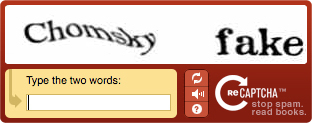
\includegraphics[scale=0.8]{images/text_image_captcha.jpg}
  \caption{Příklad obrázku, který generovala služba reCAPTCHA (verze 1) obsahující text \uv{Chomsky fake}.}
  \label{fig:captcha_text_image}
\end{figure}


\subsubsection*{Identifikace objektů v obraze}
Uživatelsky komfortnějším přístupem, jak rozlišit člověka od počítače, je zob\-razit uživateli množinu různých obrázků a požadovat výběr pouze těch, které obsahují nějaký předmět. Zaměříme-li se na technologii Google reCaptcha\footnote{\url{https://www.google.com/recaptcha/}}, lze pozorovat dva přístupy k tomuto problému. První variantou je zobrazit uživateli 9 obrázků, ze kterých je například vyžadován výběr právě takových, které obsahují dopravní značky. Druhý přístup je segmentace obrazu do několika částí a vyžadování výběru pouze těch, které obsahují určitý objekt (například auto). Využití podobného přístupu se také využívá k monetizaci obsahu majitelů webů, jelikož existují technologie používající CAPTCHA jako inzertní plochu\footnote{\url{http://confidentcaptcha.com/}}, respektive poskytují nástroj na kategorizaci velkých datasetů koncovými uživateli\footnote{\url{https://hcaptcha.com/}}. 

\begin{figure}[H]
\centering
\begin{subfigure}[b]{.5\textwidth}
  \centering
  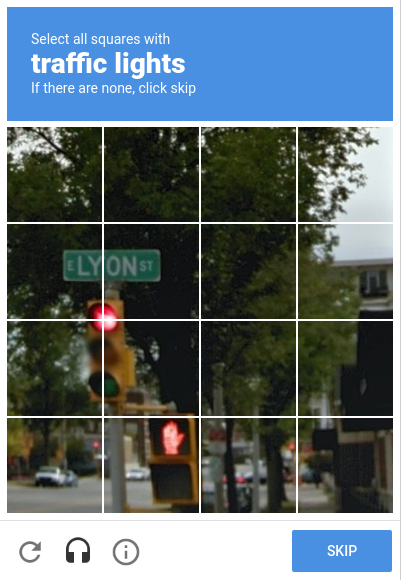
\includegraphics[width=.8\linewidth]{images/squares.png}
  \caption{Výběr dlaždic obsahujících semafor.}
  \label{fig:recaptcha_selection}
\end{subfigure}%
\begin{subfigure}[b]{.5\textwidth}
  \centering
  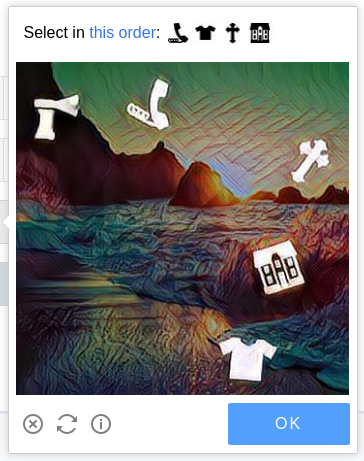
\includegraphics[width=.8\linewidth]{images/geetest_select.png}
  \caption{Výběr objektů v daném pořadí.}  \label{fig:geetest_selection}
\end{subfigure}
\caption{Příklady CAPTCHA vyžadující označení specifických objektů.}
\label{fig:image_selection}
\end{figure}

\subsubsection*{noCAPTCHA}
Ve snaze snížit interakci s uživatelem na minimum a tím i zvýšit komfort užívání webových stránek, byly vyvinuty tzv. \textit{noCAPTCHA} typy. 
Ukázkou takového přístupu je \textit{No CAPTCHA reCAPTCHA} či \textit{GeeTest Click}. V případě zmíněných typů musí návštěvník pouze kliknout na tlačítko. Veškerá verifikace uživatele je poté provedena na pozadí s využitím analýzy různých příznaků. Těmi mohou být cesta myši, doba kliku, otisk prohlížeče, atd. V případě nedostatečné jistoty je zobrazena složitější výzva.

\begin{figure}[H]
\centering
\begin{subfigure}[b]{.5\textwidth}
  \centering
  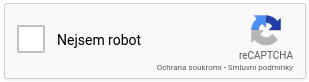
\includegraphics[width=.8\linewidth]{images/nocaptcha.png}
  \caption{No CAPTCHA reCAPTCHA}
  \label{fig:sub1}
\end{subfigure}%
\begin{subfigure}[b]{.5\textwidth}
  \centering
  
\includegraphics[width=.8\linewidth]{images/geetest_click.png}
  \caption{GeeTest Click}
  \label{fig:sub2}
\end{subfigure}
\caption{Příklady CAPTCHA vyžadující minimální interakci s uživatelem.}
\label{fig:test}
\end{figure}

\subsubsection*{Skládání puzzle}
Další variantou CAPTCHA technologie pracující s obrazem nazvěme skládáním puzzle (společnost \textit{GeeTest} používá anglický název \uv{Slide}), což znázorňuje obrá\-zek \ref{fig:captcha_geetest}. Přístup spočívá v~přesunu části obrazu ve tvaru dílku puzzle zpět na své původní místo pomocí posuvníku. Během procesu ověření je sledováno několik faktorů ovlivňujících vyhodnocovací proces, stejně jako v předchozím uvedeném typu.

\begin{figure}[H]
  \centering
  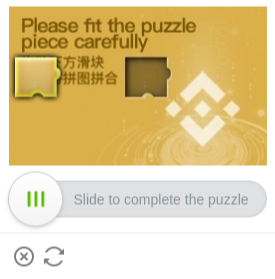
\includegraphics[scale=0.7]{images/geetest.png}
  \caption{Varianta GeeTest Slide používaná na webu \url{binance.com}}
  \label{fig:captcha_geetest}
\end{figure}

\subsubsection*{Audio CAPTCHA}
Zabezpečení pomocí textové/obrazové verifikace má nevýhodu v obtížném vyplňováním osobami se zrakovým postižením. Právě proto je vhodné takovým uživatelům nabídnout alternativní možnost (ikonu obecně užívanou pro audio lze nalézt v obrázcích \ref{fig:captcha_text_image} nebo \ref{fig:recaptcha_selection}) ověření, aby mohli využívat chráněné služby. Často se~tomu děje pomocí tzv. audio CAPTCHA, kdy jsou v nahrávce zakódovány znaky abecedy a uživatel je vyzván k jejich přepisu. V audionahrávkách lze nalézt jisté metody zkreslující zvuk, aby bylo možné předejít automatizovanému zpracování.

\subsection{Možnosti prolamování}
\subsubsection*{Nalezení chyby v implementaci}
Triviálním způsobem prolomení CAPTCHA kódů je využít chyby v implementaci generování výzev. Uživatel, který si řiká Ak1T4, popisuje\footnote{\url{https://medium.com/bugbountywriteup/bypassing-captcha-like-a-boss-d0edcc3a1c1}} vložení zahashované hodnoty odpovědi do formuláře spolu s typem obrázkové CAPTCHA. Využitím vhodných nástrojů a rainbow tabulek (tabulka obsahující dva sloupce -- plain text a příslušnou hash) je možné s odpovídajícím hardwarem nalézt rychle správnou odpověď.

\subsubsection*{Outsourcing rozpoznání}
Stále používanou variantou automatického rozpoznávání CAPTCHA kódů je~pro\-nájem služeb třetích stran\footnote{\url{https://anti-captcha.com}}$^{,}$\footnote{\url{https://2captcha.com}}. Jde o webové služby, které typicky prostřednictvím svého API nabízejí placejícím zákazníkům rozpoznání reálným pracovníkem. Výhodou rozpoznání člověkem je adaptace na možné změny v typu zabez\-pe\-čení zaručující zachování míry úspěšnosti. Avšak morálně pochybným faktem je, že tyto služby využívají pracovníky z rozvojových zemí (například Venezuely, Indonésie, Vietnamu, atd.), kteří jsou ohodnoceni velmi nízkou mzdou (hodinová sazba se uvádí v rozpětí 0,2 USD až 0,8 USD). 

\subsubsection*{Strojové učení}
V závěru se dostáváme k metodám, které jsou z informatického pohledu zajímavé. Díky pokroku oboru strojového učení a kvalitě softwaru umožňujícího s technikami oboru pracovat, je možné nechat vykonat práci rozpoznání CAPTCHA, kterou prováděl v předchozím odstavci lidský pracovník, strojem. Techniky se~zejména liší v přístupu, jaké druhy kódů lze rozpoznávat. Zatímco \cite{43464} se snaží o~vytvoření univerzálního algoritmu prolamujícího co největší množství různých CAPTCHA kódů, \citep{Kopp2016HowTM} naopak přistupuje k problému minimalisticky a jednoduchou metodou rozpoznává konkrétní typy kódů.
\newpage
\section{Captcha Breaker}
Cílem diplomové práce je kromě stručného úvodu do problematiky CAPTCHA zabezpečení také demonstrace možnosti jeho prolamování. Jako vhodný typ se jeví rozpoznání zkresleného textu v obraze. Jelikož hlavní inspirace pocházela z \cite{Kopp2016HowTM}, některé typy CAPTCHA vybrané k prolomení byly zvoleny shodné, aby bylo možné porovnat úspěšnost odlišných postupů rozpoznání extrahovaných symbolů. Aplikace demonstruje prolamování na typech CAPTCHA vyskytujících se na webech:
\begin{description}[align=left]
\item [\href{https://adiseet.mfcr.cz}{adiseet.mfcr.cz}] Daňový portál Finanční správy České republiky.
\begin{figure}[H]
  \centering
  
\includegraphics[scale=0.5]{images/eet.png}
\end{figure}

\item [\href{https://kamody.cz}{kamody.cz}] Zástupce typického internetového e-shopu.
\begin{figure}[H]
  \centering
  
\includegraphics{images/kamody.jpg}
\end{figure}

\item [\href{https://mojedatovaschranka.cz}{mojedatovaschranka.cz}] Portál určený pro elektronickou komunikaci s úřady.\footnote{V průběhu tvorby diplomové práce došlo k zásadní aktualizaci webové aplikace \url{https://mojedatovaschranka.cz} a původní CAPTCHA zabezpečení bylo nahrazeno technologií Google reCAPTCHA.}
\begin{figure}[H]
  \centering
  
\includegraphics[scale=0.5]{images/datovka.png}
\end{figure}

\item [\href{https://telerik.com}{telerik.com}] Framework pro plantformu ASP.NET.
\begin{figure}[H]
  \centering
  
\includegraphics{images/telerik.jpg}
\end{figure}

\item  [\href{https://ulozto.cz}{ulozto.cz}] Oblíbená služba pro sdílení souborů.
\begin{figure}[H]
  \centering
  
\includegraphics{images/ulozto.jpg}
\end{figure}
\end{description}


Jelikož je uživatelská příprava datasetu poměrně náročný úkol, kromě zmíně\-ného algoritmu byla vytvořena webová aplikace, která umožňuje spustit průvodce tvorby datasetu nebo klasifikátoru. Zároveň je na stejném webu možné zkusit rozluštit známé typy CAPTCHA schémat. 

\subsection{Použité technologie}
\subsubsection*{Python}
Populární interpretovaný jazyk podporující různá programovací paradigmata. V~současnosti se řadí mezi 
nejpopulárnější programovací jazyky\footnote{\url{https://insights.stackoverflow.com/survey/2019}}, zároveň v~ob\-lasti strojového učení poskytuje všechny potřebné knihovny. Nevýhodou jazyka je obtížnost paralelního zpracování dat, což je řešeno knihovnami třetích stran.

\subsubsection*{Flask}
Flask je microframework určený pro tvorbu webových aplikací napsaný v jazy\-ce Python. Samotné jádro frameworku v základu obsahuje s nadsázkou pouze ná\-stroje pro směrování požadavků a šablonovací systém Jinja. Vyžadujeme-li funk\-cio\-nalitu navíc (například komunikaci s DB, ORM mapování, validaci formulářů nebo autentizaci požadavků), je nutné doinstalovat patřičný modul. Framework se tedy snaží být minimalistický a je pouze na uvážení vývojáře, jaké moduly k~jádru frameworku dodá. 
\subsubsection*{PostgreSQL}
Pro perzistentní uložení informací bylo nutné zvolit některý z relačních databázových systémů. V aplikace bylo zvoleno PostgreSQL, zejména kvůli jeho popularitě a podpoře JSON datového typu. 
\subsubsection*{Celery}
Důležitým požadavkem pro některé aplikace je možnost vykonávat některé ope\-race asynchronně. K tomu lze v případě Flasku, respektive Pythonu obecně, použít knihovnu Celery. Jedná se o distribuovaný systém sloužící pro zpracování zasílaných zpráv, které jsou předávány skrze nějakého z podporovaných prostředníků, tzv. brokerů. I když primárně míří na zpracování v reálném čase, podporuje například zařazení obdržených zpráv do fronty a jejich sekvenční zpracování.

Knihovna umožňuje spustit libovolnou Python metodu jako úlohu v separátním vlákně, je-li obalena tzv. dekorátorem \texttt{@celery.task}. V aplikaci je takové chování využito k předání informací o klasifikátoru, který je potřeba natrénovat.

\subsubsection*{RabbitMQ}
Jako broker pro komunikaci s Celery byl použit RabbitMQ. Jedná se o úložiště pracující primárně v operační paměti, nicméně lze jej nakonfigurovat tak, aby ukládal data na pevný disk a po restartu zařízení byl schopen obnovit svůj stav.

\subsubsection*{PyTorch}
Open-source knihovna zaměřená na strojové učení v jazyce Python. Byť se jedná o volbu méně populární než například TensorFlow\footnote{\url{https://towardsdatascience.com/deep-learning-framework-power-scores-2018-23607ddf297a}}, pro potřeby vyvinuté aplikace je plně dostačující.


\subsubsection*{jQuery}
jQuery je již několik let nejpoužívanější javascriptovou knihovnou\footnote{\url{https://w3techs.com/technologies/overview/javascript\_library/all}} vůbec. Mezi její silné stránky patří snadná manipulace s DOM nebo obsluha AJAX requestů. Těchto vlastností využívá zejména průvodce tvorbou datasetu v administrační části aplikace.

\subsubsection*{Bootstrap}
Spolu s jQuery tvoří CSS knihovna Bootstrap základ velkého množství webů. Programátor je s jejím použítím odstíněn od nutnosti stylovat prvky webové stránky a je možné se více soustředit na samotný vývoj backendu.

\subsection{Uživatelská část}
Část aplikace dostupná neautorizovanému uživateli obsahuje výčet známých typů CAPTCHA kódů, které je možné prolomit spolu s formulářem pro nahrání uživatelova obrázku. Po výběru obrázku k prolomení a příslušného klasifikátoru, je možné zaslat dotaz na server, který z obrázku dekóduje znaky pomocí vybraného klasifikátoru, což je řešeno asynchronním dotazem na backend aplikace. Nastane-li chyba, je uživateli zobrazena příslušná hláška. V případě úspěšného rozpoznání pouze obsah dekódovaný ze zaslaného obrázku.

Zasílaný dotaz na server obsahuje pouze dva parametry - ID klasifikátoru a~obrázek zakódovaný do Base64. Jakmile server obdrží požadavek, nejprve zkontroluje existenci klasifikátoru. Pokud přijal špatnou hodnotu, informuje o takové situaci uživatele chybovou odpovědí. Následně jsou z vstupního obrázku extrahovány jednotlivé symboly dle konfigurace datasetu zvoleného klasifikátoru. V~posledním kroku jsou extrahované symboly předány klasifikátoru k rozpoznání. V odpovědi je poté předána dekódovaná hodnota.

\begin{figure}[H]
  \centering
  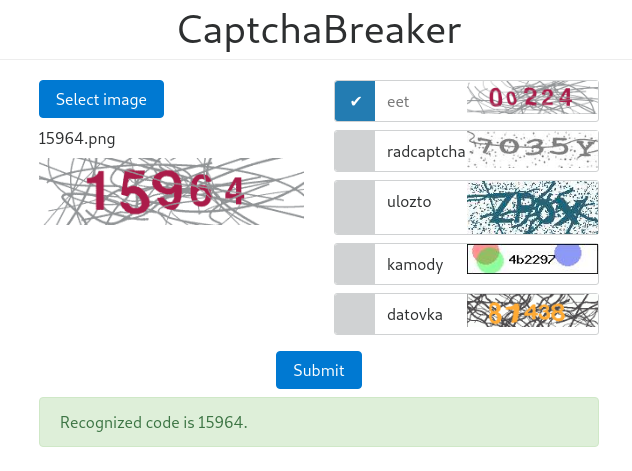
\includegraphics[scale=0.6]{images/website_public.png}
  \caption{Rozpoznaný kód.}
  \label{fig:resolved}
\end{figure}

\begin{minipage}[t]{0.45\textwidth}
\begin{verbatim}
{
"message":
"Unknown classifier",
"status":
"error"
}
\end{verbatim}
Chybová odpověď
\end{minipage}
\begin{minipage}[t]{0.45\textwidth}
\begin{verbatim}
{
"message":
"15964",
"status":
"success"
}
\end{verbatim}
Odpověď v případě rozpoznání znaků
\end{minipage}

\begin{table}[H]
\centering
\begin{tabular}{|l|l|l|}
\hline
\textbf{URL} & \textbf{metoda} & \textbf{význam}
\\ \hline
\texttt{/} & \texttt{GET} & domovská stránka uživatelské části
\\ \hline
\texttt{/decode/} & \texttt{POST} & AJAX dekódování CAPTCHA
\\ \hline
\end{tabular}
\caption{URL endpointy pro globální namespace}
\end{table}

\subsection{Administrační rozhraní}
Část webu dostupná pouze administrátorovi je dostupná na URL \texttt{/dashboard}. Všechny dotazy přicházející na adresy v tomto jmenném prostoru musejí být autentizovány. Jelikož jde pouze o demonstrativní webovou aplikaci, není zde řešen přístup několika autorizovanými uživateli, případně různé víceúrovňové kontroly přístupu. Přihlašovací údaje jsou kontrolovány vůči konstantám \texttt{APP\_USERNAME}, respektive \texttt{APP\_PASSWORD} v konfiguračním souboru aplikace. Bezpečnost ta\-ko\-vého přístupu lze dále zvýšit například restrikcí IP adres u dotazů přicházející na chráněné endpointy v konfiguraci použitého aplikačního serveru.

\subsubsection*{Nástěnka \texttt{/dashboard/overview/}}
 Na nástěnce jsou zobrazeny statistiky příchozích dotazů na rozpoznání obsahu CAPTCHA obrázků a počtu datasetů, resp. klasifikátorů. Existují-li navíc klasifikátory, které se momentálně trénují, jsou na nástěnce zobrazeny informace o stavu procesu. Kromě názvu klasifikátoru je zobrazeno pořadí aktuální iterace, respektive informace o fázi verifikace. Data o trénovaných klasifikátorech jsou pravidelně aktualizována v intervalu 5 vteřin pomocí AJAX dotazů. Po natrénování klasifikátoru je informace o něm z nástěnky odstraněna.

\subsubsection*{Nahrání datasetu \texttt{/dashboard/datasets/new/}}
Proces nahrání datasetu je zahrnut v jednoduchém průvodci. Administrátor je nejprve vyzván k vybrání ZIP archivu se vzorovými CAPTCHA obrázky. Následně je mu umožněno přiřadit jednotlivým obrázkům texty, které jsou v~nich obsaženy. V případě vynechání tohoto kroku se význam textů určuje podle názvu souborů. V posledním kroku je konfigurace grafických operací (obrázek \ref{fig:dataset_new}), které zkonvertují vstupní obraz do podoby vhodné pro extrahování symbolů. Jakmile je administrátor spokojený s výsledkem, odešle dataset na server a je přesměrován na stránku s jeho detaily.

\begin{figure}[h]
  \centering
  \includegraphics[scale=1]{images/datasets_new.png}
  \caption{Konfigurace extrakce symbolů z datasetu.}
  \label{fig:dataset_new}
\end{figure}

\subsubsection*{Zobrazení datasetu \texttt{/dashboard/datasets/:id/}}
Stručný přehled s informacemi o vytvořeném datasetu. V horní části stránky jsou zobrazeny informace o času vytvoření, obsažených znacích a celkovém počtu rozpoznaných symbolů. Následuje výpis nahraných obrázků spolu se zobrazením extrahovaných symbolů. V poslední části je vypsána konfigurace extrakce ve~formátu JSON. 

\subsubsection*{Tvorba klasifikátoru \texttt{/dashboard/classificators/new/}}
Formulář konfigurace klasifikátoru je parametrizován šesti vstupy - názvem klasifikátoru, zdrojovým datasetem, maximálním počtem iterací, velikostí \textit{learning rate}, velikostí \textit{momentum} a případým nastavením křížové validace. Po odeslání požadavku na vytvoření klasifikátoru je samotná fáze trénování spuštěna v asynchronním procesu na pozadí a administrátor je přesměrován na nástěnku, kde vidí průběžně aktualizované informace o trénování klasifikátoru.

\subsubsection*{Detaily klasifikátoru \texttt{/dashboard/classificators/:id/}}
Stránka zobrazuje detaily konfigurace klasifikátoru spolu s informací o jeho konfiguraci. Po natrénování klasifikátoru je možné získat informace o hodnotách ztrátové funkce, respektive úspěšnosti křížové validace.

\subsection{Podporované grafické operace}
Aplikace momentálně podporuje několik grafických operací, které slouží k pří\-pravě obrazu, ze kterého jsou extrahovány jednotlivé symboly. Jejich použití je nutné vzhledem k možnému použití metod, které zkreslují znaky zanesené do~obrazu. Architektura aplikace je navržena tak, že jsou jednotlivé třídy grafic\-kých operací automaticky převoditelné do HTML kódu včetně svých argumentů. Zároveň implementují vlastní (de)se\-riali\-zaci, což umožňuje snadnou rozšiřitelnost webového průvodce tvorbou data\-setu.
\subsubsection*{Stupně šedi (Grayscale)}
Operace převádějící obraz z RGB spektra do stupňů šedi.
\begin{figure}[H]
\centering
\begin{subfigure}{.5\textwidth}
  \centering
  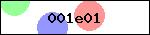
\includegraphics[width=.8\linewidth]{images/grayscale_original.jpg}
\end{subfigure}%
\begin{subfigure}{.5\textwidth}
  \centering
  
\includegraphics[width=.8\linewidth]{images/grayscale_result.png}
\end{subfigure}
\caption{Vlevo původní obrázek, vpravo po černobílá verze po transformaci.}
\label{fig:crop_example}
\end{figure}

\subsubsection*{Oříznutí (Crop)}
V některých případech obsahuje vstupní obraz rámeček, který bez odstranění způsobuje selhání algoritmu nalezení největších ploch. Z toho důvodu byla při\-dána možnost oříznout vstupní obraz rovnoměrně ze všech stran.

\begin{table}[H]
\centering
\begin{tabular}{|l|l|l|l|}
\hline
\textbf{Název argumentu} & \textbf{typ} & \textbf{význam}
\\ \hline
size & \texttt{Integer} & velikost ořezu
\\ \hline
\end{tabular}
\caption{Argumenty operace oříznutí.}
\end{table}

\begin{figure}[H]
\centering
\begin{subfigure}{.5\textwidth}
  \centering
  
\includegraphics[width=.8\linewidth]{images/crop_original.png}
\end{subfigure}%
\begin{subfigure}{.5\textwidth}
  \centering
  
\includegraphics[width=.8\linewidth]{images/crop_result.png}
\end{subfigure}
\caption{Vlevo původní obrázek, vpravo po aplikaci operace oříznutí.}
\label{fig:crop_example}
\end{figure}

\subsubsection*{Otsovo prahování (Otsu's treshold)}
Otsovo prahování se používá k automatickému převodu obrazu z odstínů šedi do~binární černobílé podoby. Interně Otsovo prahování analyzuje histogram vstup\-ního obrazu, dle kterého určuje následné rozdělení na popředí/pozadí obrazu. 


\begin{figure}[H]
\centering
\begin{subfigure}{.5\textwidth}
  \centering
  
\includegraphics[width=.8\linewidth]{images/otsu_original.png}
\end{subfigure}%
\begin{subfigure}{.5\textwidth}
  \centering
  
\includegraphics[width=.8\linewidth]{images/otsu_result.png}
\end{subfigure}
\caption{Vlevo původní obrázek, vpravo po aplikaci Otsova prahování.}
\label{fig:inverse_example}
\end{figure}

\subsubsection*{Inverze (Inverse)}
Inverze v aplikaci slouží k záměně popředí/pozadí obrazu. V některých případech užití Otsova prahování totiž dojde k jevu, kdy je část obrazu, která je hledaná v~segmentačním algoritmu, označena jako pozadí. Jelikož je na vstupu očekávaný binární obraz, operace je implementována jako bitová negace.
\begin{figure}[H]
\centering
\begin{subfigure}{.5\textwidth}
  \centering
  
\includegraphics[width=.8\linewidth]{images/inverse_original.png}
\end{subfigure}%
\begin{subfigure}{.5\textwidth}
  \centering
  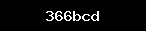
\includegraphics[width=.8\linewidth]{images/inverse_result.png}
\end{subfigure}
\caption{Vlevo původní obrázek, vpravo po aplikaci inverze.}
\label{fig:inverse_example}
\end{figure}

\subsubsection*{Uživatelské prahování (Custom treshold)}
Operace uživatelského prahování slouží k definování rozsahu hodnot pixelů, které jsou následně označeny jako popředí/pozadí a podle kterých je vstupní obraz převede do binární podoby. Operace je užitečná u typů CAPTCHA schémat, kdy je potřeba zachovat pouze části obrazu určité barvy. V případě použití Otsova prahování může totiž dojit k zachování nežádoucího šumu.

\begin{table}[H]
\centering
\begin{tabular}{|l|l|l|l|}
\hline
\textbf{Název argumentu} & \textbf{typ} & \textbf{význam}
\\ \hline
lower\_bound & \texttt{Integer} & spodní hranice hodnot popředí
\\ \hline
upper\_bound & \texttt{Integer} & horní hranice hodnot popředí
\\ \hline
\end{tabular}
\caption{Argumenty uživatelského prahování.}
\end{table}


\begin{figure}[H]
\centering
\begin{subfigure}{.5\textwidth}
  \centering
  
\includegraphics[width=.8\linewidth]{images/custom_original.png}
\end{subfigure}%
\begin{subfigure}{.5\textwidth}
  \centering
  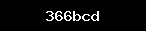
\includegraphics[width=.8\linewidth]{images/custom_result_0_50.png}
\end{subfigure}
\caption{Vlevo původní obrázek, vpravo po aplikaci uživatelského prahování v rozsahu $0 - 50$.}
\label{fig:inverse_example}
\end{figure}

\subsubsection*{Odstranění spojitých ploch (Area Filter)}
Jedná se o pomocnou operaci, jejímž účelem je komfortnější obsluha průvodce tvorby datasetu. Operace odstraní plochy obrazu, které mají svou plochu menší než je uživatelem definovaná velikost, případně je jejich výška menší než definované velikost. Důsledkem je odfiltrování šumu z obrazu bez nutnosti použití morfologických operací, které by mohly s příliš vysokými argumenty nevhodně poškodit obraz.
\begin{figure}[H]
\centering
\begin{subfigure}{.5\textwidth}
  \centering
  
\includegraphics[width=.8\linewidth]{images/filter_original.png}
\end{subfigure}%
\begin{subfigure}{.5\textwidth}
  \centering
  
\includegraphics[width=.8\linewidth]{images/filter_result.png}
\end{subfigure}
\caption{Vlevo původní obrázek, vpravo po odstranění spojitých ploch.}
\label{fig:inverse_example}
\end{figure}
\subsubsection*{Morfologické transformace}
Před samotným výčtem morfologických operací je vhodné zmínit, o jaký proces se jedná. Morfologická operace očekává na vstupu dva argumenty -- obrázek a~strukturální element (také nazývaný jádro). Pro zjednodušení uvažujme pouze binární obrázky, ačkoliv lze operace zobecnit také na barevné. Jádro i obrázek lze vyjádřit jako matice (v aplikaci je vždy použita čtvercová matice) s hodnotami z množiny $ {0, 1} $. Jádro je posouváno nad jednotlivými pixely vstupního obrázku, jejíž hodnotu mění dle dále popsaných vlastností. Samotné jádro je možné určit několika tvary. Jedná se o 
\begin{enumerate*}[label={\alph*)}]
\item kříž
\item kruh nebo
\item čtverec.
\end{enumerate*}
Všechny varianty jádra velikosti $5 \times 5$ jsou vyobrazeny níže. Zároveň mají všechny morfologické operace shodné argumenty.


$$
\begin{bmatrix} 
0 & 0 & 1 & 0 & 0 \\
0 & 0 & 1 & 0 & 0 \\
1 & 1 & 1 & 1 & 1 \\
0 & 0 & 1 & 0 & 0 \\
0 & 0 & 1 & 0 & 0 \\
\end{bmatrix}
\quad
\begin{bmatrix} 
0 & 0 & 1 & 0 & 0 \\
0 & 1 & 1 & 1 & 0 \\
1 & 1 & 1 & 1 & 1 \\
0 & 1 & 1 & 1 & 0 \\
0 & 0 & 1 & 0 & 0 \\
\end{bmatrix}
\quad
\begin{bmatrix} 
1 & 1 & 1 & 1 & 1 \\
1 & 1 & 1 & 1 & 1 \\
1 & 1 & 1 & 1 & 1 \\
1 & 1 & 1 & 1 & 1 \\
1 & 1 & 1 & 1 & 1 \\
\end{bmatrix}
$$

\begin{table}[H]
\centering
\begin{tabular}{|l|l|l|l|}
\hline
\textbf{Název argumentu} & \textbf{typ} & \textbf{význam}
\\ \hline
kernel\_size & \texttt{Integer} & velikost jádra $2 * kernel\_size + 1$
\\ \hline
iterations & \texttt{Integer} & počet iterací operace
\\ \hline
kernel\_shape & \texttt{ENUM}  & tvar jádra
\\ \hline
\end{tabular}
\caption{Argumenty morfologických operací.}
\end{table}

\begin{figure}[H]
\centering
\begin{subfigure}{.5\textwidth}
  \centering
  
\includegraphics[width=.8\linewidth]{images/kernel_square.png}
\end{subfigure}%
\begin{subfigure}{.5\textwidth}
  \centering
  
\includegraphics[width=.8\linewidth]{images/kernel_cross.png}
\end{subfigure}
\caption{Vlevo morfologické otevření s jádrem tvaru \texttt{čtverec}, vpravo stejná operace s jádrem tvaru \texttt{kříž}. Symbol \texttt{5} je vlevo poškozený.}
\label{fig:inverse_example}
\end{figure}

\subsubsection*{Morfologická eroze (Morphological erosion)}
Hodnota pixelu pod středem jádra zůstává zachována, jsou-li všechny pixely pod nenulovými body jádra také nenulové. V tomto případě dochází k odfiltrování šumu, vyhlazení hran a odstranění hrany obrazu.
\begin{figure}[H]
\centering
\begin{subfigure}{.5\textwidth}
  \centering
  
\includegraphics[width=.8\linewidth]{images/erosion_original.png}
\end{subfigure}%
\begin{subfigure}{.5\textwidth}
  \centering
  
\includegraphics[width=.8\linewidth]{images/erosion_result.png}
\end{subfigure}
\caption{Vlevo původní obrázek, vpravo po aplikaci morfologické eroze.}
\label{fig:inverse_example}
\end{figure}

\subsubsection*{Morfologická dilatace (Morphological dilation)}
Dilatace představuje opačnou operaci k erozi. Hodnota pixelu pod středem jádra zůstává zachována, je-li alespoň jeden pixel pod nenulovými body jádra také nenulový. Dochází k rozšíření hran obrazu, případně zaplnění mezery mezi blízkými částmi obrazu.
\begin{figure}[H]
\centering
\begin{subfigure}{.5\textwidth}
  \centering
  
\includegraphics[width=.8\linewidth]{images/dilation_original.png}
\end{subfigure}%
\begin{subfigure}{.5\textwidth}
  \centering
  
\includegraphics[width=.8\linewidth]{images/dilation_result.png}
\end{subfigure}
\caption{Vlevo původní obrázek, vpravo po aplikaci morfologické dilatace.}
\label{fig:inverse_example}
\end{figure}

\subsubsection*{Morfologické uzavření (Morphological closing)}
Dilatace následovaná erozí. Nejprve jsou okraje obrazu rozšířeny a zaplněny případné mezery, poté obraz eroduje a zmenši okraje na původní velikost.
\begin{figure}[H]
\centering
\begin{subfigure}{.5\textwidth}
  \centering
  
\includegraphics[width=.8\linewidth]{images/closing_original.png}
\end{subfigure}%
\begin{subfigure}{.5\textwidth}
  \centering
  
\includegraphics[width=.8\linewidth]{images/closing_result.png}
\end{subfigure}
\caption{Vlevo původní obrázek, vpravo po aplikaci morfologického uzavření.}
\label{fig:inverse_example}
\end{figure}

\subsubsection*{Morfologické otevření (Morphological opening)}
V posledním případě jde o erozi následovanou dilatací. Po odfiltrování šumu a~vyhlazení hran okraje obrazu dilatují do původních hodnot.
\begin{figure}[H]
\centering
\begin{subfigure}{.5\textwidth}
  \centering
  
\includegraphics[width=.8\linewidth]{images/opening_original.png}
\end{subfigure}%
\begin{subfigure}{.5\textwidth}
  \centering
  
\includegraphics[width=.8\linewidth]{images/opening_result.png}
\end{subfigure}
\caption{Vlevo původní obrázek, vpravo po aplikaci morfologického otevření.}
\label{fig:inverse_example}
\end{figure}

\subsubsection*{Škálování (Scale)}
Operace zvětšující obraz celočíselným koeficientem. Jelikož mají morfologické operace v některých situacích na obrázcích s příliš nízkým rozlišením příliš destruktivní charakter, je vhodné vstupní obrázek zvětšit a provést několik iterací dané operace.

\begin{table}[H]
\centering
\begin{tabular}{|l|l|l|l|}
\hline
\textbf{Název argumentu} & \textbf{typ} & \textbf{význam}
\\ \hline
scale\_ratio & \texttt{Integer} & koeficient škálování
\\ \hline
\end{tabular}
\caption{Argumenty operace škálování.}
\end{table}


\subsection{Extrakce symbolů}
Extrakce symbolů se provádí nad obrázky z uživatelem nahraného datasetu v~podobě ZIP archivu. Podporovány jsou všechny obrazové formáty, které podporuje knihovna OpenCV. Ke spuštění extrakce je také potřeba informace o~počtu hledaných symbolů v obraze a konfigurace zpracování obrazu. Volitelně je na\-hrán také slovník přiřazující jednotlivým souborům význam symbolů v nich uložených. Výsledkem jsou extrahované jednotlivé znaky do unifikovaného rozměru  $20\times20$ pixelů, které se následně ukládají do databáze.

\subsubsection*{Možné kolize}
Během procesu extrakce symbolů jsou v obraze hledány spojité plochy pixelů, které mohou představovat symbol CAPTCHA kódu. Ne vždy je však ihned nalezeno požadované množství takových oblastí. 
\begin{itemize}
\item \textbf{Byl nalezen velký počet spojitých ploch.} Proces předzpracování ob\-razu nemusí v některých případech vyčistit obraz v žádoucí kvalitě a proto může být nalezeno více ploch, spojitých ploch obrazu, které lze považovat za symbol. V takovém případě se pro každou takovou oblast vypočítá její velikost a zachová se pouze $n$ největších, kde $n$ značí počet hledaných symbolů.

\item \textbf{Byl nalezen malý počet spojitých ploch.} Některé CAPTCHA obrázky mohou být natolik deformovány, že se symboly v nich obsažené navzájem prolínají. Takovou vadu lze například odstranit spočítáním tzv. lokálních minim v jednotlivých spojitých plochách. Každé takové lokální minimum se označí hodnotou určující rovnoměrnost rozdělení obsaženého symbolu. Dokud není určeno $n$ oblastí obsahující symbol, vybere se a rozdělí taková spojitá plocha, jejíž ohodnocení rozdělení je maximální.
\end{itemize}


\subsection{Tvorba klasifikátoru}
Klasifikátorem se rozumí algoritmus, jehož účelem je přiřadit vstupnímu prvku správnou kategorii na základě trénovacích dat, se kterými byl algoritmus trénován. Konkrétně v případě rozpoznání symbolů v navrženém algoritmu se jedná o~při\-řazení indexu v poli známých symbolů datasetu. Klasifikátor může být implementován různými způsoby. Vyvinutá aplikace používá konvoluční neuronovou síť, jejíž architektura je patrná z příslušné třídy. 

\subsubsection*{Umělá neuronová síť}
Velmi populární výpočetní model v oblasti umělé inteligence představuje tzv. umělá neuronová síť. Ta je složena z jednotlivých umělých neuronů poskládaných do vícero vrstev a jedná se, neformálně řečeno, o počítačovou simulaci biolo\-gické neuronové sítě. V případě vícevrstvých neuronových sítí jsou velmi často konstruovány tzv. plně propojené neuronové sítě. V takovém případě jsou vý\-stupy všech neuronů jedné vrstvy použity jako vstup každého neuronu vrstvy následující.

Umělý neuron lze popsat jako entitu definovanou svými vstupy $x_i$, ohodnocením vstupních hodnot $w_i$, prahovou hodnotou aktivace neuronu $\Theta$ a přenosovou funkcí $\varphi(x)$. Hodnota výstupu umělého neuronu je dána $\varphi(\sum_{i=1}^{N}x_i * w_i)$. 

Příkladem přenosové funkce je \textit{skoková funkce}, pro kterou platí $\varphi(x) = 0$ pro $x < \Theta$, resp. $\varphi(x) = 1$ pro $x \geq \Theta$. Další populární variantou je funkce $sigmoid$, jejíž hodnota je dána rovnicí $\varphi(x) = \frac{1}{1-e^{-x}}$.

\subsubsection*{Trénování umělých neuronových sítí}
Má-li umělá neuronová síť sloužit ke klasifikaci dat, je nutné po zadefinování její architektury projít procesem trénování. Trénování neuronové sítě je proces, během kterého jsou optimalizovány váhy vstupů jednotlivých neuronů do~takové podoby, aby v konečném důsledku produkovala neuronová síť relevantní odpovědi. S omezením na variantu trénování s učitelem (existuje také varianta trénování bez učitele) lze konstatovat, že jedním z nejpoužívanějších učících algoritmů je tzv. \textit{gradient descent}. Určuje-li tzv. \textit{loss function} odchylku neuronové sítě od~správného řešení, \textit{gradient descent} se snaží její hodnotu snížit na minimum. Po každém průchodu algoritmu nad trénovacími daty jsou upraveny váhy $w_i$ jednotlivých neuronů v závislosti na odchylce od správného řešení. Hodnotu, o~kterou jsou $w_i$ upraveny, lze ovládat parametrem \textit{learning rate} a nazvěme ji krok sestupu. U nastavení parametru \textit{learning rate} je vhodné být obzvlášť opatrný. Příliš velká hodnota může vést k nenalezení optimálních vah neuronové sítě, malá hodnota naopak vede k pomalé adaptaci. 

Algoritmus \textit{gradient descent} lze rozšířit o techniku nazvanou \textit{momentum}. Tato technika umožňuje rychlejší trénování neuronové sítě na základě úpravy směru sestupu. Směr sestupu je upraven v případě, že je v historii jednotlivých kroků sestupu nalezen například určitý vzorec oscilace.


\subsubsection*{Konvoluční neuronová síť}
Speciální typ umělých neuronových sítí jsou konvoluční neuronové sítě, které jsou optimalizovány pro práci s obrazovými daty. Nevýhodou klasických neuronových sítí je narůstající počet neuronů v případě architektury sítě s několika skrytými vrstvami, respektive nedetekování hledaného vzoru v případě jeho posunu v obraze. V kontextu této práce není druhý problém příliš relevantní, jelikož jsou vstupní data normalizována.

Architekturu konvolučních neuronových sítí je možné rozdělit do tří částí. První z nich jsou konvoluční vrstvy. Nad vstupním obrazem je možné provést libovolnou konvoluční operaci. Její výsledek je někdy nazýván jako filtr.

Další částí je tzv. \textit{pooling} vrstva, která redukuje rozměr každého filtru. Běžně se využívá operace nazývaná \texttt{MaxPool2D}. Průběh operace lze chápat jako posouvání čtvercové matice dimenze $n*n$ nad filtrem, kdy se do výstupního filtru propíše pouze maximální hodnota pod posuvnou maticí.

Poslední částí je plně propojená vrstva, které agreguje jednotlivé filtry z pooling vrstvy s použitím různých aktivačních funkcí. Jedná-li se o agregaci informací z filtrů, použije se \textit{ReLU} aktivační funkce, v případě finální klasifikace funkce \textit{softmax}.

\subsubsection*{Křížová validace}
Křížovou validací se rozumí metoda ověření přesnosti výsledků trénovaného klasifikátoru. Vstupní data jsou rozdělena do $k$ disjunktních množin stejné velikosti. Následně je každá z těchto množin uvažována jako testovací a se zbylými je natrénován klasifikátor. Výsledkem je $k$ hodnot udávající úspěšnost správné klasifikace dat z trénovací množiny.

\subsection*{Konfigurace klasifikátoru}
V rozhraní aplikace je pro uživatele připravena stránka pro konfiguraci klasifikátoru, kterému je možné nastavit parametry omezující počet iterací, určit velikost \textit{learning rate}, \textit{momentum} a případně zapnout vyko\-nání křížové validace. Doba trénování klasifikátoru se odvíjí od použitého hardwaru, lze však konstatovat, že vytvořit klasifikátor pro použité datasety trvá maximálně několik minut.

\subsection{Úspěšnost implementované metody prolamování}
Pro ověření úspěšnosti navržené metody prolamování CAPTCHA kódů bylo z~webů uvedených v úvodu kapitoly staženo a manuálně označeno 400 různých obrázků, ze kterých byly vytvořeny datasety. Množství trénovacích dat se může na první pohled zdát být malé v porovnání s populárním datasetem obsahujícím ručně psané číslice MNIST \citep{mnist}, avšak podle výsledků křížové validace je pro účely diplomové práce postačující. Výsledky uvedené v tabulce \ref{succesful_rate_mine} prezentují průměrnou hodnotu křížové validace pro $k=5$. Podrobnější informace může čtenář získat přímo ve webové aplikaci.

\begin{table}[H]
\centering
\begin{tabular}{|l|l|}
\hline
\textbf{Název webu} & \textbf{Úspěšnost}
\\ \hline
adiseet.mfcr.cz & 0,9610
\\ \hline
kamody.cz & 0,9983
\\ \hline
mojedatovaschranka.cz & 0,9915
\\ \hline
telerik.com & 0,7705
\\ \hline
ulozto.cz & 0,3568
\\ \hline
\end{tabular}
\caption{Úspěšnost rozpoznání jednotlivých symbolů CAPTCHA kódů metodou navrženou v této práci.}
\label{succesful_rate_mine}
\end{table}

Porovnáme-li úspěšnosti rozpoznání symbolů v tabulce \ref{succesful_rate_mine} oproti tabulce \ref{succesful_rate_mimic}, lze pozorovat mírný nárůst úspěšnosti prolamování, resp. klasifikace konvoluční neuronovou sítí oproti algoritmu k-NN. Je vhodné podotknout, že podmínky za~kterých byla zjišťována úspěšnost metod prolamování, nebyly shodné. Zatímco tato diplomová práce provádí vždy křížovou validaci s $k=5$ nad datasetem obsahující 400 označených obrázků, \citep{Kopp2016HowTM} používá křížovou validaci s $k=10$. V~případě zabezpečení na webu \url{http://mojedatovaschranka.cz} byl použit znatelně menší dataset obsahující pouze 50 označených obrázků. 

Jelikož obě metody používají velmi podobný druh předzpracování obrazu, lze usuzovat, že rozdíl v úspěšnosti rozpoznání dat je dán použitým klasifikátorem. Z experimentů provedených s datasetem MNIST \citep{mnist} je možné sledovat podobný rozdíl v úspěšnosti klasifikátoru k-NN a konvoluční neuronové sítě.

\begin{table}[H]
\centering
\begin{tabular}{|l|l|}
\hline
\textbf{Název webu} & \textbf{Úspěšnost}
\\ \hline
mojedatovaschranka.cz & 0,82
\\ \hline
ulozto.cz & 0,14
\\ \hline
\end{tabular}
\caption{Úspěšnost rozpoznání jednotlivých symbolů CAPTCHA kódů v \citep{Kopp2016HowTM}.}
\label{succesful_rate_mimic}
\end{table}

Zároveň lze pozorovat patrný význam aplikace zkreslujících křivek na popředí CAPT\-CHA typu použitého na webu \url{https://adiseet.mfcr.cz}. V porov\-nání s ob\-rázky použitými na webu \url{https://mojedatovaschranka.cz}, kde je CAPTCHA typ až na~umístění zkreslujících křivek shodný, dochází k poklesu úspěšnosti rozpoznání přibližně o  tři procenta.

\subsection{Další vývoj}
Ultimativní nástroj pro lámání CAPTCHA kódů, byť pouze obrázkových, nebyl vytvořen. Implementace následujících funkcionalit, zejména v administračním rozhraní, by výrazně zlepšila komfort užívání a zřejmě i praktičnost systému jako celku.

\subsubsection*{Upozornění na chybně klasifikované znaky} 
Na stránce zobrazující detaily klasifikátoru se naskýtá možnost zobrazit upozornění na možné chybně klasifikované symboly. Taková chyba může nastat zej\-ména v následujících třech případech: 
\begin{itemize}
\item Příliš podobné znaky (číslice 0 versus písmeno O).
\item Algoritmus pro extrakci symbolů na výstupu nevrátí celý znak, ale napří\-klad pouze jeho část.
\item Symbol byl ručně chybně označen a klasifikátor jej rozpoznává správně.
\end{itemize}

\subsubsection*{Změna označení již nahraných obrázků} 
Během procesu vytváření datasetu musí administrátor nahrát ZIP archiv obsahující obrázky jejichž název odpovídá CAPTCHA kódu, nebo je procesem označení obrázků proveden před uploadem na server. V obou případech však závisí jen a~pouze na lidském faktoru, zda bude obrázku přiřazen správný nebo chybný text. Z toho důvodu je vhodné umožnit změnu označení obrázku, resp. samotného symbolu.

\subsubsection*{Odstranění některých znaků}
V některých případech není možné segmentovat jednotlivé symboly z datasetu se stoprocentní úspěšností. Aby se trénovaná neuronová síť neučila na chybně označených datech, je vhodné umožnit odstranit z datasetu ty symboly, které byly špatně extrahovány.

\subsubsection*{Volba z více klasifikátorů} 
V současné době systém používá jako klasifikátor konvoluční neuronovou síť. Takový klasifikátor nemusí vyhovovat všem rozpoznávaným typům CAPTCHA obrázků. Rovněž pro účely porovnání úspěšnosti různých klasifikátorů je rozumné přidat možnost volby.

\subsubsection*{Klasifikátor používající více datasetů} 
K dalšímu zlepšení rozpoznávání by mohlo také vést trénování klasifikátoru znaky z více zdrojů. Kromě primárního datasetu, který udává i proces extrakce symbolů, by k jeho množině znaků byly přidány ty symboly s odpovídající hodnotou ze~zvolených datasetů. Tím by se docílilo rozpoznání transformací, které v trénovací množině symbolů nebyly prve zahrnuty.


%% Závěry práce. V jazyce práce a anglicky. Text pro jiný než
%% nastavený jazyk práce (nepovinným parametrem language makra
%% \documentclass, výchozí český) se zadává použitím makra s uvedením
%% jazyka jako nepovinného parametru.
\begin{kiconclusions}
Vyvinutá webová aplikace úspěšně prolamuje některé typy známých CAPTCHA kódů. Existuje však mnoho prostoru pro další vývoj, který by usnadnil rozpoz\-návání dalších typů zabezpečení. Retrospektivně je také vhodné zmínit, že volba frameworku Flask se zdá být velice nešťastná vzhledem k ne příliš pohodlné práci s objektově-relačním mapováním nebo tvorbě administračního rozhraní. Přepsání webové aplikace například do Ruby on Rails se zachováním části obstarávající strojové učení v jazyce Python by mohlo být optimálnější pro snadnou udržitelnost aplikace.
\end{kiconclusions}

\begin{kiconclusions}[english]
Developed web application succesfully breaks certain types of known CAPTCHA codes. However there is many possibilities of further development, which would make recongizing of other security types easier.  It is also worth mentioning that retrospecively the choice of the Flask framework seems to be very unfortune due to not so comfortable work with object-relational mapping or creation of administration interface. Rewriting the code base of web application e.g. into Ruby on Rails with retaining machine learning part in Python language would be more feasible because of better sustainability of the application. 
\end{kiconclusions}

%% Přílohy obsahu textu práce, za makrem \appendix.
\appendix

%% Obsah přiloženého CD/DVD. Poslední příloha. Upravte podle vlastní
%% práce!
\section{Obsah přiloženého CD/DVD} \label{sec:ObsahCD}

\begin{description}

\item[\texttt{doc/}] \hfill \\
  Text práce ve formátu PDF, vytvořený s~použitím závazného stylu KI
  PřF UP v~Olomouci pro závěrečné práce, včetně všech příloh,
  a~všechny soubory potřebné pro bezproblémové vygenerování PDF
  dokumentu textu (v~ZIP archivu), tj.~zdrojový text textu, vložené
  obrázky, apod.

\item[\texttt{src/}] \hfill \\
  Kompletní zdrojové texty webové aplikace \textsc{CaptchaBreaker} se všemi potřebnými (příp.~převzatými) knihovnami. Dostupné také z \url{https://github.com/arthurwozniak/CaptchaBreaker}.

\end{description}

U~veškerých cizích převzatých materiálů obsažených na CD/DVD jejich
zahr\-nutí dovolují podmínky pro jejich šíření nebo přiložený souhlas
držitele copyrightu. Pro všechny použité (a~citované) materiály,
u~kterých toto není splněno a~nejsou tak obsaženy na CD/DVD, je uveden
jejich zdroj (např.~webová adresa) v~bibliografii nebo textu práce
nebo v souboru \texttt{readme.txt}.

%% -------------------------------------------------------------------

%% Sazba volitelného seznamu zkratek, za přílohami.
\printglossary

%% Sazba povinné bibliografie, za přílohami (případně i za seznamem
%% zkratek). Při použití BibLaTeXu použijte makro
%% \printbibliography. jinak prostředí thebibliography. Ne obojí!

%% Sazba i v textu necitovaných zdrojů, při použití
%% BibLaTeXu. Volitelné.
\nocite{*}
%% Vlastní sazba bibliografie při použití BibLaTeXu.
\printbibliography

%% Bibliografie, včetně sazby, při nepoužití BibLaTeXu.
% \begin{thebibliography}{9}
%\bibitem{kniha2} \uppercase{Hawke}, Paul. NanoHttpd: Light-weight HTTP server designed for embedding in other applications. GitHub [online]. 2014-05-12. [cit. 2014-12-06]. Dostupné z: \url{https://github.com/NanoHttpd/nanohttpd}
%
%\bibitem{jeske13} \uppercase{Jeske}, David; \uppercase{Novák}, Josef. Simple HTTP Server in \csharp: Threaded synchronous HTTP Server abstract class, to respond to HTTP requests. CodeProject: For those who code [online]. 2014-05-24. [cit. 2014-12-06]. Dostupné z: \url{http://www.codeproject.com/Articles/137979/Simple-HTTP-Server-in-C}
%
%\bibitem{uzis2012} \uppercase{ÚSTAV ZDRAVOTNICKÝCH INFORMACÍ A STATISTIKY ČR}. Lékaři, zubní lékaři a farmaceuti 2012 [online]. Praha 2, Palackého náměstí 4: Ústav zdravotnických informací a statistiky ČR, 2012 [cit. 2014-12-06]. ISBN 978-80-7472-089-5. Dostupné z: \url{http://www.uzis.cz/publikace/lekari-zubni-lekari-farmaceuti-2012}
% \end{thebibliography}

%% Sazba volitelného rejstříku, za bibliografií.
\printindex

\end{document}
